\documentclass{beamer}
%\usepackage{lmodern}
\usepackage[ngerman]{babel}
\usepackage[utf8]{inputenc}
\usepackage{listings}
\usepackage{caption}

% lstlisting-Einstellungen
\lstset{
	language=Python,
	morekeywords = {yield},
	basicstyle=\ttfamily,
	keywordstyle=\color{blue}\ttfamily,
	stringstyle=\color{red}\ttfamily,
	commentstyle=\color{green}\ttfamily,
	morecomment=[l][\color{magenta}]{\#},
	% wegen Leerzeichen-Anzeige	
	showstringspaces=false,
	% wegen Character-Spacing
	columns=fullflexible,	
}

% auto-nummerierung bei framebreaks
\setbeamertemplate{frametitle continuation}{(\insertcontinuationcount)}

% nummerierung
\setbeamertemplate{footline}[frame number]{}

% kein "Abbildung: " bei figure-captions
\captionsetup[figure]{labelformat=empty}

% keine merkwürzige Toolbar unten
\beamertemplatenavigationsymbolsempty

% etwas nach links
\setlength{\leftmargini}{1em}

%%%%%%%%%%%%%%%%%%%%%%%%%%%%%%%%%%%%%%%%%%%%%%%%%%%%%%%%%%%%%%%%%%%%%%%%%%%%%%%%

\title{Scrapy}
\subtitle{A Fast and Powerful Scraping and Web Crawling Framework}
\author{MB, TS, TS}
\subject{Computer Science}

%%%%%%%%%%%%%%%%%%%%%%%%%%%%%%%%%%%%%%%%%%%%%%%%%%%%%%%%%%%%%%%%%%%%%%%%%%%%%%%%

\begin{document}

\frame{\titlepage}
\begin{frame}
	\frametitle{Übersicht}
	\tableofcontents
\end{frame}
\section{Allgemeines}
\begin{frame}[fragile]
\frametitle{\insertsection{}: Definition Scaping}
		Laut Wikipedia:
		
		Der Begriff Screen Scraping [..] umfasst
		generell alle Verfahren zum Auslesen von Texten aus Computerbildschirmen. 
		Gegenwärtig wird der Ausdruck jedoch beinahe ausschließlich in Bezug auf Webseiten 
		verwendet [..]. In diesem Fall bezeichnet Screen Scraping speziell die
		Technologien, die der Gewinnung von Informationen durch gezieltes Extrahieren der benötigten Daten dienen.
\end{frame}

\begin{frame}[fragile]
\frametitle{\insertsection{}: Aha\ldots Und was ist dieses Scrapy?}
	\begin{itemize}
		\item "`A Fast and Powerful Scraping and Web Crawling Framework"'
		\item Also ein freies und open-source-Framework für Python, welches
		web-scraping beherrscht.
		\item https://scrapy.org/
	
	\end{itemize}
\end{frame}

%%%%%%%%%%%%%%%%%%%%%%%%%%%%%%%%%%%%%%%%%%%%%%%%%%%%%%%%%%%%%%%%%%%%%%%%%%%%%%%%

\section{Installation}
% fragile nötig für listings
\begin{frame}[fragile]
	\frametitle{\insertsection}
	\begin{itemize}
		\item mit pip (erfordert vorhandene Python-Installation):
			\begin{lstlisting}
pip3 install scrapy
			\end{lstlisting}
		\item mit anaconda (in Windows einfacher, da numpy, etc... bereits enthalten):
			\begin{lstlisting}
conda install -c conda-forge scrapy
			\end{lstlisting}
	\end{itemize}
\end{frame}

\section{Extraktion von Daten}
\begin{frame}[fragile,allowframebreaks]
	\frametitle{\insertsection{}}
	\begin{lstlisting}[basicstyle=\footnotesize]
<div class="quote">
    <span class="text">"The world as we have..."</span>
    <small class="author">Albert Einstein</small>
</div>
<div class="quote">
    <span class="text">"It is our choices,..."</span>
    <small class="author">J.K. Rowling</small>
</div>
...
	\end{lstlisting}
	%\framebreak	
	\begin{lstlisting}[breaklines=true,basicstyle=\footnotesize]
def parse(self, resp):
  res1 = resp.css('div small')
  #[<Selector data='<small...">'>, <Selector data='<small...">'>, ...]
  res2 = resp.css('div small::text')
  #[<Selector data='Albert Einstein'>, <Selector data='J.K. Rowling'>, ...]
  res3 = resp.css('div small::text').extract()
  #['Albert Einstein', 'J.K. Rowling', ...]
  res4 = resp.css('div small::text').extract_first()
  #Albert Einstein
	\end{lstlisting}
	

	
	\framebreak
	
	\begin{itemize}
		\item \lstinline|resp.css('div small')| selektiert mehrere Elemente im DOM
		mit dem CSS-Selektor \lstinline|'div small'| (d.h. es findet alle \lstinline|<small>|-Elemente innerhalb von \lstinline|<div>|-Elementen)
		\item \lstinline|resp.css('div small::text')| selektiert den Text innerhalb jedes gefundenen \lstinline|<small>...</small>|-Tags
		\item \lstinline|resp.css('div small::text').extract()| liefert die selektierten Texte als Liste von Python-Strings
		\item \lstinline|resp.css('div small::text').extract_first()| liefert den 1. Treffer davon
	\end{itemize}
	
	\framebreak
	
	\begin{itemize}
		\item das Ergebnis einer Selektion kann selbst wieder zum Selektieren genutzt werden
		\item folgendes Beispiel selektiert alle Zitate einer Website, und gibt je Zitat als Datensatz Autor und Wortlaut zurück:
	\begin{lstlisting}
def parse(self, response):
  quotes = response.css('div.quote')
  for q in quotes:
    yield {
      'author': q.css('.author::text').extract_first(),
      'text': q.css('.text::text').extract_first()
    }
	\end{lstlisting}
	\end{itemize}
\end{frame}

\section{Shell}
\subsection{Vorfühurng: E-mails farmen\ldots}
\begin{frame}[fragile]
	\frametitle{\insertsection{}: \insertsubsection{}}
	\begin{itemize}
		\item In der ersten Übung wollen wir uns zunächst mit einigen Befehlen von
		Scrapy in der Shell vertraut machen.
		\item Die Aufgabe besteht darin die E-mails der HSNR-Dozenten von der
		offiziellen Homepage zu crawlen.
		\begin{itemize}
			\item Dazu müssen wir scrapy zunächst mitteilen, mit welcher Website wir
			arbeiten wollen: 

			\begin{lstlisting}  
scrapy shell 'https://www.hs-niederrhein.de/
elektrotechnik-informatik/personen/'
			\end{lstlisting}
			
			bzw. unter Windows:
			
			\begin{lstlisting}  
scrapy shell "https://www.hs-niederrhein.de/
elektrotechnik-informatik/personen/"
			\end{lstlisting}
						

		\end{itemize}
	\end{itemize}
\end{frame}

\framebreak


\begin{frame}[fragile]
	\frametitle{\insertsection{}: \insertsubsection{}}
	\begin{itemize}
		\item Anschließend schauen wir uns den HTML-Code der entsprechenden Seite an
		und überlegen uns, auf welche Elemente wir zugreifen müssen.
		\item Offensichtlich besteh die Dozentenliste aus einer Reihe von
		div-Containern in denen die Personendaten enthalten sind. Wir greifen mittels 
			\begin{lstlisting}  
response.css("div.tx-iwpersonen-pi1-item-box")
			\end{lstlisting}
		auf die entsprechenden Container zu und erhalten eine Liste der div-Elemente
		als Ausgabe.
		\item Diese kann natürlich auch in eine Variable gespeichert werden\ldots
		\begin{lstlisting}  
persons = response.css(...)
			\end{lstlisting}
	\end{itemize}
\end{frame}

\framebreak

\begin{frame}[fragile]
	\frametitle{\insertsection{}: \insertsubsection{}}
	\begin{itemize}
		\item Um an die E-mail-Adressen zu kommen, müssen wir nun noch einmal in den
		Quellcode schauen.
		\item Anscheinend sind die E-Mailadressen als Link mit dem
		CSS-Klassenselektor "`font-size-11"' hinterlegt.
		\item \begin{lstlisting}  
persons.css("a.font-size-11::text").extract()
			\end{lstlisting}
			liefert dann eine Liste der E-mailadressen zurück.
		\item Nun müssen wir nur noch das (at) durch ein @-Zeichen ersetzen und können
		anschließend die Liste verwenden um liebe Rundmails zu versenden. ;-)
	\end{itemize}
\end{frame}

\framebreak

\begin{figure}
	\begin{center}
		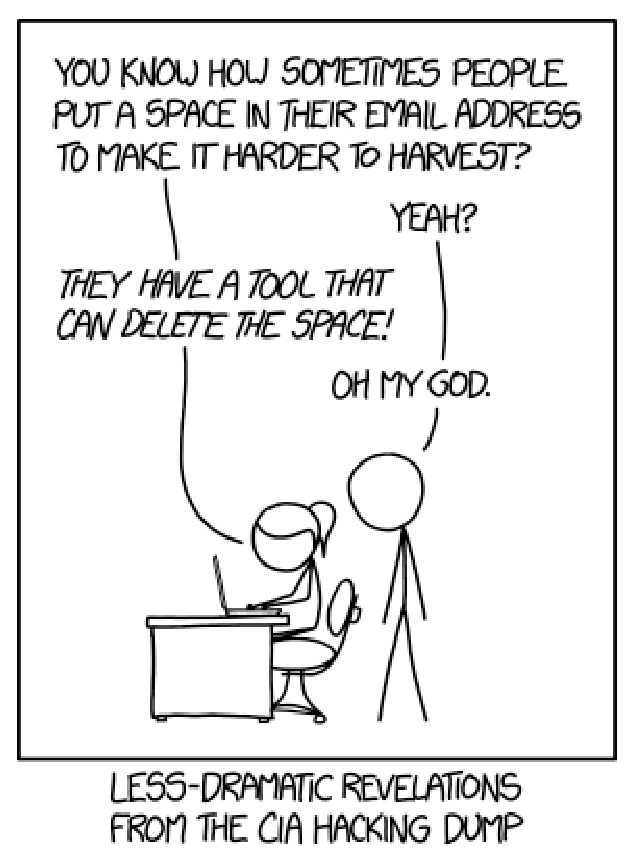
\includegraphics[width=0.6\textwidth]{texsrc/hacking_xkcd}
	\end{center}
	\label{fig:XKCD_HACKING}
\end{figure}

\begin{frame}[fragile,allowframebreaks]
	\frametitle{\insertsection{}: \insertsubsection{} Kommandos als Spider}

\begin{lstlisting}  
import scrapy

class MailSpider(scrapy.Spider):
  name = "emails"
  start_urls = [
    'https://www.hs-niederrhein.de/
    elektrotechnik-informatik/personen/',
  ]

  def parse(self, response):
    persons = response.css(
      "div.tx-iwpersonen-pi1-item-box")


    for person in persons:
      mail = person.css("a.font-size-11::text")
        .extract_first();
      name = person.css(
        "a.tx-iwpersonen-pi1-detaillink::text").extract_first();
      mail = mail.replace("(at)", "@")
      yield{name : mail,}
      \end{lstlisting}
\end{frame}

\section{Projekt anlegen}
\begin{frame}[fragile]
	\frametitle{\insertsection}
	\begin{itemize}
		\item Verzeichnisstruktur erzeugen:
			\begin{lstlisting}
scrapy startproject mynewproject
			\end{lstlisting}
		\item erzeugt ein gleichnamiges Verzeichnis \verb|./mynewproject| 
		\item künftige Spider werden in \verb|./mynewproject/spiders| angelegt
		\item Konfiguration erfolgt über \verb|./mynewproject/settings.py|
		\begin{itemize}
		  \item ermöglicht z.B. Konfiguration der Beachtung von \lstinline|robots.txt|
  		\end{itemize}
	\end{itemize}
\end{frame}

%%%%%%%%%%%%%%%%%%%%%%%%%%%%%%%%%%%%%%%%%%%%%%%%%%%%%%%%%%%%%%%%%%%%%%%%%%%%%%%%

\section{Spider}
\begin{frame}[fragile]
	\frametitle{\insertsection}
	\begin{itemize}
		\item spezielle Klassen in Scrapy-Projekten
		\item von Klasse \verb|scrapy.Spider| abgeleitet
		\item führen Crawling durch, spezifisch für Websites programmierbar
		\item Ablauf: \begin{enumerate}		
			\item Spider schickt Requests an initiale URLs
			\item scrapy ruft je Response Callback-Methode auf, mit Inhalt als Parameter
			\item Callback-Methode startet ggf. Requests an weitere URLs
			\item Callback-Methode extrahiert Daten des Response und gibt sie zurück
			\item scrapy sammelt alle zurückgegebenen Daten ein, und speichert sie z.B. in einer Datei
		\end{enumerate}
	\end{itemize}
\end{frame}

%%%%%%%%%%%%%%%%%%%%%%%%%%%%%%%%%%%%%%%%%%%%%%%%%%%%%%%%%%%%%%%%%%%%%%%%%%%%%%%%

\begin{frame}[fragile]
	\frametitle{Spider?}	
	\begin{figure}
		\begin{center}
			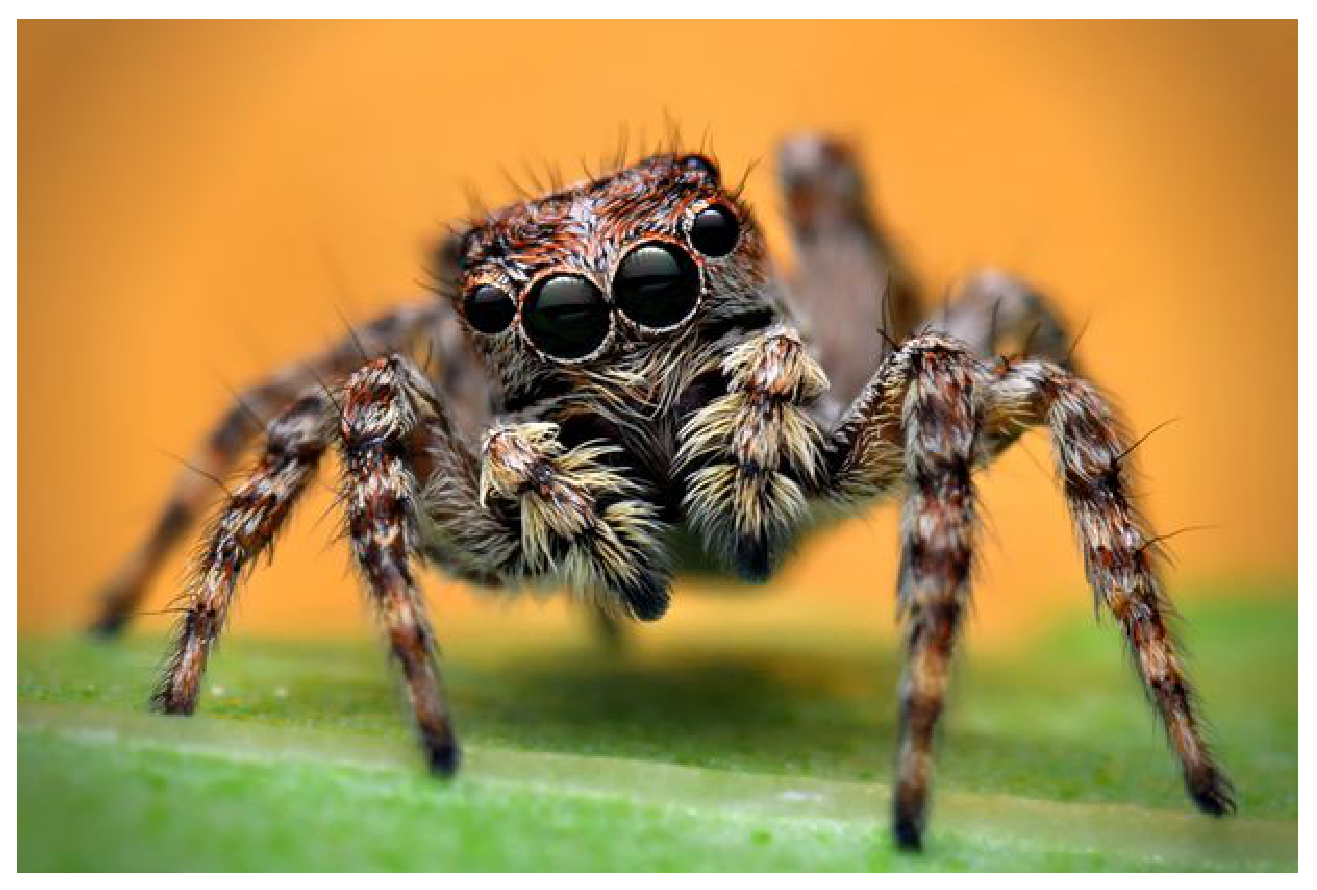
\includegraphics[width=0.6\textwidth]{texsrc/Spider_cute}
		\end{center}
		%\vspace{-10pt}
		\caption{Spider! Funfact: Spinne ist im Volksmund ein Synonym für Tiere aus
		der Gruppe der Arachnide - kleine Tiere mit acht Beinen, welche Insekten mit Netzen oder
		anderen Fallen fangen.}
		\label{fig:Spider}
	\end{figure}
\end{frame}

%%%%%%%%%%%%%%%%%%%%%%%%%%%%%%%%%%%%%%%%%%%%%%%%%%%%%%%%%%%%%%%%%%%%%%%%%%%%%%%%

\begin{frame}[fragile,allowframebreaks]
	\frametitle{einfacher Beispielspider}
			\begin{lstlisting}
import scrapy

class SimpleSpider(scrapy.Spider):
    name = 'simplespider'
    start_urls = ['http://supersimpleloremipsum.com/']

    def parse(self, response):
        self.logger.info('parsing {}'.format(response))
        yield {'status': response.status}
			\end{lstlisting}
			
	\framebreak
	
	\begin{itemize}
		\item \lstinline|name| identifiziert den Spider eindeutig im Projekt
		\item \lstinline|start_urls| beinhaltet die URLs für die initialen Requests
		\item \lstinline|parse()| wird als Callback aufgerufen, der Parameter \lstinline|response| enthält das Ergebnis des Response
		\item die Methode erzeugt eine Logging-Ausgabe von \lstinline|response| 
		\item die Methode übergibt scrapy das Parsingergebnis den HTTP-Statuscode als \lstinline|dict|
	\end{itemize}
	
	\framebreak
	
%%%%%%%%%%%%%%%%%%%%%%%%%%%%%%%%%%%%%%%%%%%%%%%%%%%%%%%%%%%%%%%%%%%%%%%%%%%%%%%%
	
	\begin{itemize}
		\item das Crawling mit Spider \lstinline|simplespider| wird über einen eigenen Befehl in der Kommandozeile gestartet:
			\begin{lstlisting}
scrapy crawl simplespider -o res.json
			\end{lstlisting}
		\item scrapy speichert die per \lstinline|yield| zurückgegebenen Daten in der Datei \lstinline|res.json| (das Dateiformat ergibt sich aus Suffix) \begin{itemize}
			\item scrapy unterstützt neben json weitere Formate: xml, csv, ... 
			\item beachte: scrapy leert bei mehrfachem Start des Crawlingbefehls die Datei nicht, sondern hängt die Daten hinten dran
		\end{itemize}
		\item Befehl auch über Pythonskript aufrufbar: \begin{lstlisting}
		
		\item TODO fix this -> new, main
		\end{lstlisting}
def main():
  cmd = 'scrapy crawl iter -o res.json'
  scrapy.cmdline.execute(cmd.split())
main()		
		\end{lstlisting}
		\item API zum Crawlen: Fehlanzeige ?
	\end{itemize}
\end{frame}

%%%%%%%%%%%%%%%%%%%%%%%%%%%%%%%%%%%%%%%%%%%%%%%%%%%%%%%%%%%%%%%%%%%%%%%%%%%%%%%%






\section{Links folgen}
\begin{frame}[fragile,allowframebreaks]
	\frametitle{\insertsection{}}
	\begin{lstlisting}
def parse(self, response):
  for q in response.css('div.quote'):
    yield {
      'text': q.css('.text::text').extract_first(),
      'author': q.css('.author::text').extract_first()
    }
  a_selector = 'li.next a::attr(href)'
  hrefs = response.css(a_selector).extract()  
  for href in hrefs:    
    yield response.follow(href, callback=self.parse)
	\end{lstlisting}
	\begin{itemize}
		\item die Methode liefert zunächst von den Zitaten Autor und Wortlaut
		\item danach sucht sie alle passenden \lstinline|<a href=...>|-Elemente und selektiert je Treffer das \lstinline|href|-Attribut mit \lstinline|'a::attr(href)'| 
		
		\framebreak
		
%%%%%%%%%%%%%%%%%%%%%%%%%%%%%%%%%%%%%%%%%%%%%%%%%%%%%%%%%%%%%%%%%%%%%%%%%%%%%%%%

		\item zuletzt extrahiert die Methode die enthaltenen URLs und untersucht sie rekursiv mit \lstinline|response.follow(href, callback=self.parse)| 
		\item scrapy speichert intern fingerprints von besuchten URLs zur Vermeidung von ``crawling loops'' \begin{itemize}
			\item Verhalten über \lstinline|DUPEFILTER_CLASS| in Konfigurationsdatei änderbar
		\end{itemize}
	\end{itemize}
\end{frame}

%%%%%%%%%%%%%%%%%%%%%%%%%%%%%%%%%%%%%%%%%%%%%%%%%%%%%%%%%%%%%%%%%%%%%%%%%%%%%%%%

\section{Übung}




%%%%%%%%%%%%%%%%%%%%%%%%%%%%%%%%%%%%%%%%%%%%%%%%%%%%%%%%%%%%%%%%%%%%%%%%%%%%%%%%
%%%%%%%%%%%%%%%%%%%%%%%%%%%%%%%%%%%%%%%%%%%%%%%%%%%%%%%%%%%%%%%%%%%%%%%%%%%%%%%%
%%%%%%%%%%%%%%%%%%%%%%%%%%%%%%%%%%%%%%%%%%%%%%%%%%%%%%%%%%%%%%%%%%%%%%%%%%%%%%%%

\subsection{Blog-Posts}
\begin{frame}
	\frametitle{\insertsection{}: \insertsubsection{}}	
	$\rightarrow$ Texte befreien! und\ldots ja was eigentlich :?
\end{frame}

%%%%%%%%%%%%%%%%%%%%%%%%%%%%%%%%%%%%%%%%%%%%%%%%%%%%%%%%%%%%%%%%%%%%%%%%%%%%%%%%
%%%%%%%%%%%%%%%%%%%%%%%%%%%%%%%%%%%%%%%%%%%%%%%%%%%%%%%%%%%%%%%%%%%%%%%%%%%%%%%%
%%%%%%%%%%%%%%%%%%%%%%%%%%%%%%%%%%%%%%%%%%%%%%%%%%%%%%%%%%%%%%%%%%%%%%%%%%%%%%%%


\subsection{Linkcounter}
\begin{frame}[fragile]
	\frametitle{\insertsection{}: \insertsubsection{}}
	\begin{itemize}
		\item Erstellung eines Scrapy-Spiders, der alle Vorkommen von in Fefes Blog
		verlinkten Domains zählt: \begin{itemize}
			\item der Spider soll in der Ausgabedatei (beliebiges Format) eine Datenstruktur als Dictionary anlegen: \begin{lstlisting} 
{
  "www.spiegel.de": 1234,
  "www.heise.de": 567,
  ...
}
			\end{lstlisting}
		\item eine Unterscheidung von \lstinline|"www.spiegel.de"| und \lstinline|"spiegel.de"| muss hier nicht vorgenommen werden (d.h. 2 Einträge sind ok)
		\item der Hostname eines Links kann z.B. mithilfe der Funktion \lstinline|urlparse| aus dem Modul \lstinline|urllib.parse| bestimmt werden
		\item nur die Links aus eigentlichen Inhalten (d.h. kein Impressum, FAQ,
		[l]-Links o.Ä.) sollen gezählt werden
		\item die Einträge sollen absteigend sortiert sein
		\end{itemize}
	\end{itemize}
\end{frame}

%%%%%%%%%%%%%%%%%%%%%%%%%%%%%%%%%%%%%%%%%%%%%%%%%%%%%%%%%%%%%%%%%%%%%%%%%%%%%%%%

\section{Fazit}
\begin{frame}
	\frametitle{\insertsection{}}
	\begin{itemize}
	  \item Datenzugriff mithilfe von CSS möglich $\rightarrow$ für uns weniger
	  neues zu lernen
	  \item Python Framework - BAD $\rightarrow$ kein $R$ - GOOD
	  \item Async - nicht einfach in Rahmenprogramm einzubetten, nicht dokumentiert
	  \item Spiderinterface sehr einfach
	  \item Viel automatisiert - Doppelte links
	  \item javascript handling? - Nope (- external program ``Splash'')
	  \item Scrap it all!!!
	\end{itemize}
\end{frame}

%%%%%%%%%%%%%%%%%%%%%%%%%%%%%%%%%%%%%%%%%%%%%%%%%%%%%%%%%%%%%%%%%%%%%%%%%%%%%%%%

\section{Quellen}
\begin{frame}
	\frametitle{\insertsection{}}
	\emergencystretch 1.5em
	\setbeamertemplate{bibliography item}{\insertbiblabel}
	{\small
	\begin{thebibliography}{8}
		\bibitem{scrapy tu}\url{https://doc.scrapy.org/en/latest/intro/tutorial.html}
		\bibitem{scrapy ins}\url{https://doc.scrapy.org/en/latest/intro/install.html}
		\bibitem{scrapy sp}\url{https://doc.scrapy.org/en/latest/topics/spiders.html}
		\bibitem{scrapy set}\url{https://doc.scrapy.org/en/latest/topics/settings.html}
	\end{thebibliography}
	}
\end{frame}




\end{document}
